\subsection{Große Projekte verwalten und Buchstruktur}

\begin{aufgabe}
Erstellen Sie das Grundger\"ust f\"ur eine eigene Abschlussarbeit. \TeX en
Sie daf\"ur das Layout der Beipsieldatei \texttt{book.pdf} so exakt wie
m\"oglich nach. Auf den Inhalt wird dabei keinen Wert gelegt (verwenden Sie
\texttt{Lorem Ipsum} Text), jedoch auf Titelseite, Kopf-/Fu\ss zeilen,
Seitenzahlen, Abbildung mit Verweis etc. Die Kapitel sollen als einzelne
Dateien vorliegen. Die weiteren Aufgaben dieser Section bearbeiten Sie bitte
an der erstellten Abschlussarbeit. 
\end{aufgabe}

\begin{aufgabe}
F\"ugen Sie der Abschlussarbeit im Anhang eine beliebige Seite aus Ihrem Protokoll hinzu. 
\end{aufgabe}

\begin{aufgabe}
Erm\"oglichen Sie es im Inhaltsverzeichnis per Link zu den jeweiligen Sections zu gelangen. Die Links sollen dabei einen dunklen Blauton haben.  
\end{aufgabe}

\subsection{Hyperlinks und Metadaten}
\begin{aufgabe}
F\"ugen Sie der Abschlussarbeit Metadaten zu Ihrer Person hinzu.
\end{aufgabe}

\begin{aufgabe}
Stellen Sie das Dokument so ein, dass beim \"Offnen das Inhaltsverzeichnis als Lesezeichen angezeigt wird. Die Seiten sollen Seite f\"ur Seite (kein kontinuierliches Scrollen) angezeigt werden. 	
\end{aufgabe}

\subsection{Literaturverzeichnis}
\begin{aufgabe}
Erstellen Sie eine Literaturdatenbank im \texttt{bib} Format mittels
\texttt{JabRef}. F\"ugen Sie mindestens ein Paper (z.B.\ \"uber PubMed), ein
Buch, sowie eine Ver\"offentlichung in einem Konferenzband (z.B.\ LNCS)
hinzu. Verwenden Sie Keys der Form \texttt{autor:YY}. Zitieren Sie alle
Dokumente Ihrer Literaturdatenbank in der Abschlussarbeit im Harvard Stil. Zitieren Sie das
Buch mit Verweis auf eine Seite. Zitate im Text sollen in runden Klammern
stehen. Zitate im Verzeichnis sollen folgendes Format haben:

\medskip
\noindent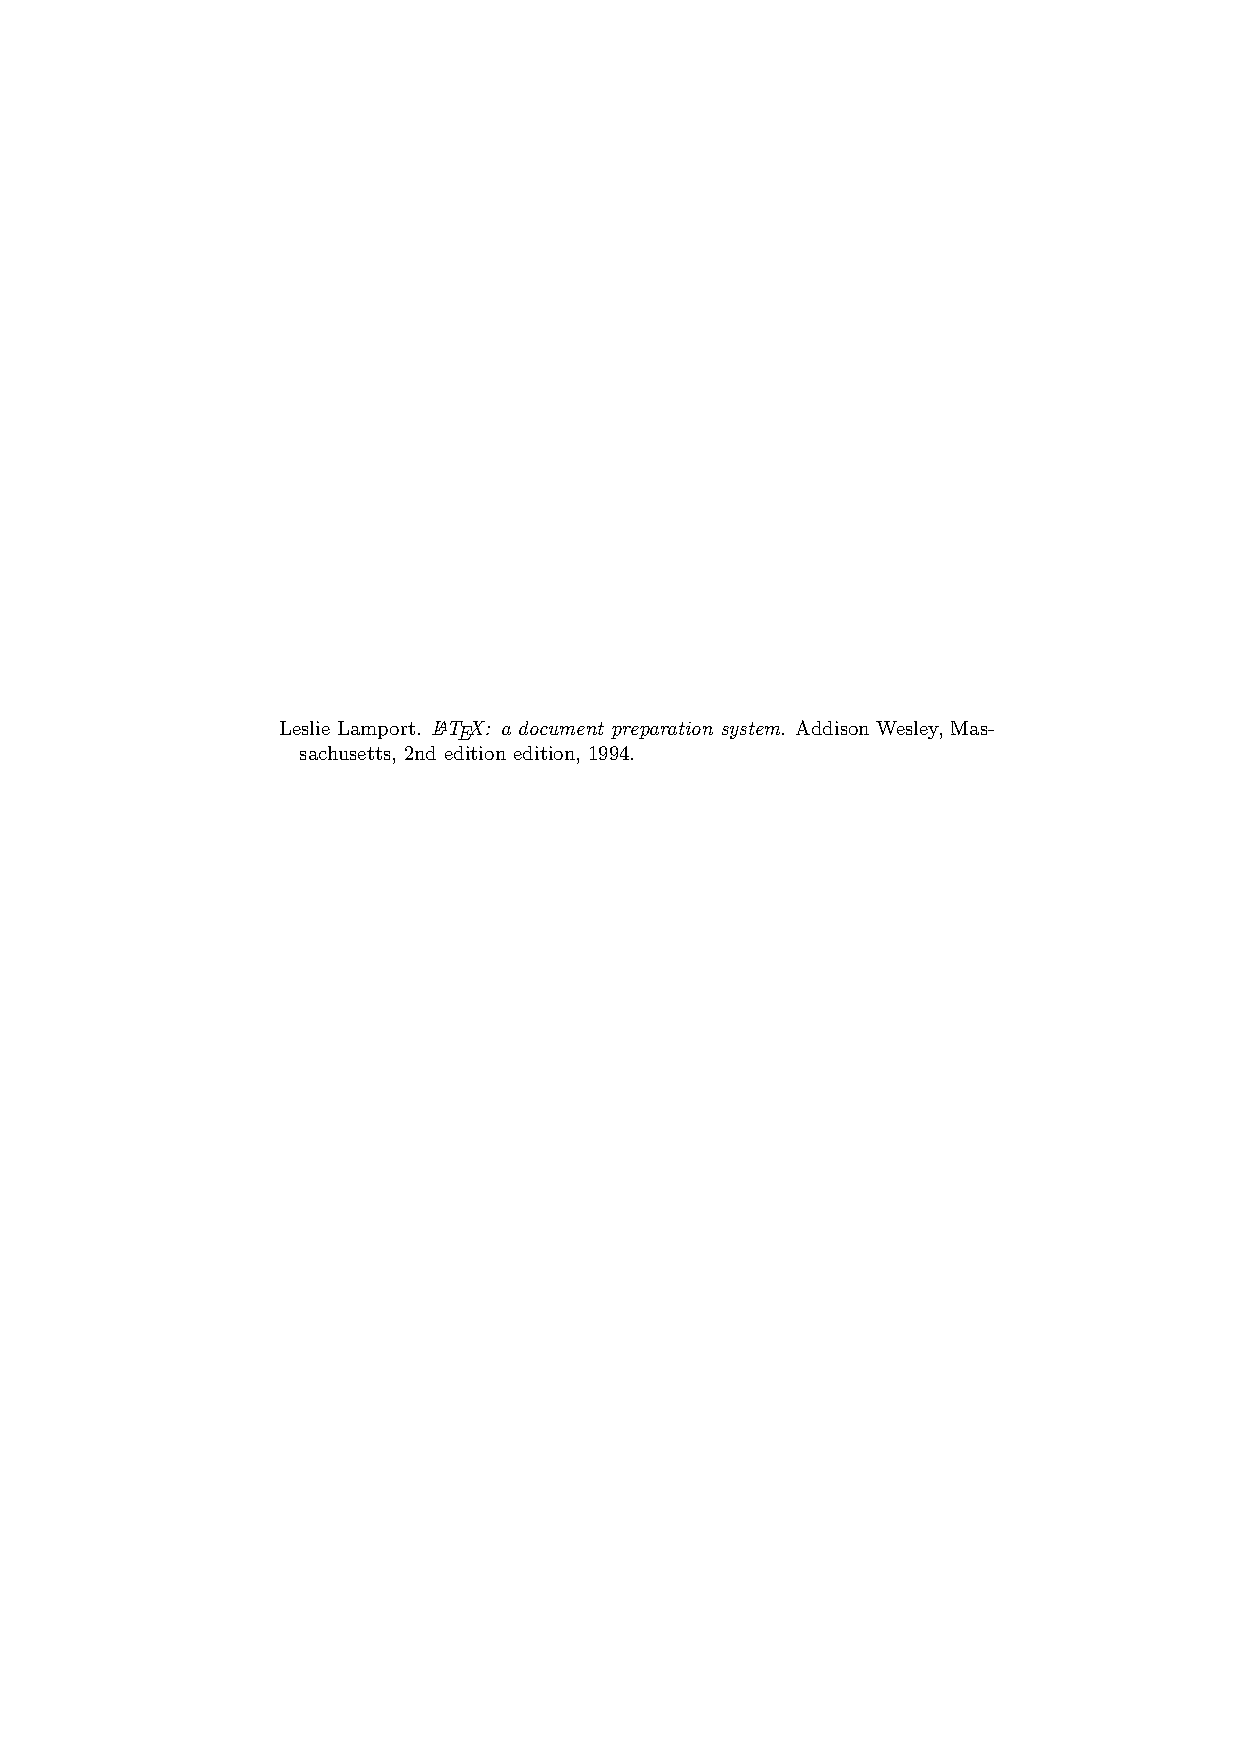
\includegraphics[width=\textwidth]{Literatur}
\end{aufgabe}
